
%----------------------------------------------------------------------------------------
%	PACKAGES AND OTHER DOCUMENT CONFIGURATIONS
%----------------------------------------------------------------------------------------

\documentclass[a4paper,12pt]{article}


%----------------------------------------------------------------------------------------
%	PACKAGES AND OTHER DOCUMENT CONFIGURATIONS
%----------------------------------------------------------------------------------------

\usepackage{amsmath,amsfonts,stmaryrd,amssymb} % Math packages

\usepackage{enumerate} % Custom item numbers for enumerations

\usepackage{mhchem}
\usepackage[hidelinks]{hyperref}
%\hypersetup{
%	colorlinks = true,
%	urlcolor=black,
%	filecolor=black,
%	citecolor=black,
%	linkcolor=black
%	}

\usepackage{multirow}
\usepackage{tabularx}
\usepackage{booktabs}
\usepackage{booktabs}
\usepackage{siunitx}
\usepackage{subfigure}
\usepackage{xcolor}

\usepackage[italian]{babel}

\usepackage[ruled]{algorithm2e} % Algorithms

\usepackage[framemethod=tikz]{mdframed} % Allows defining custom boxed/framed environments

\usepackage{listings} % File listings, with syntax highlighting
\lstset{
	basicstyle=\ttfamily, % Typeset listings in monospace font
}

\renewcommand*\figurename{Figura}
\renewcommand*\refname{Riferimenti bibliografici}

%----------------------------------------------------------------------------------------
%	DOCUMENT MARGINS
%----------------------------------------------------------------------------------------

\usepackage{geometry} % Required for adjusting page dimensions and margins

\geometry{
	paper=a4paper, % Paper size, change to letterpaper for US letter size
	top=2.5cm, % Top margin
	bottom=3cm, % Bottom margin
	left=2.5cm, % Left margin
	right=2.5cm, % Right margin
	headheight=14pt, % Header height
	footskip=1.5cm, % Space from the bottom margin to the baseline of the footer
	headsep=1.2cm, % Space from the top margin to the baseline of the header
	%showframe, % Uncomment to show how the type block is set on the page
}

%----------------------------------------------------------------------------------------
%	FONTS
%----------------------------------------------------------------------------------------

\usepackage[utf8]{inputenc} % Required for inputting international characters
\usepackage[T1]{fontenc} % Output font encoding for international characters

\mdfdefinestyle{commandline}{
	leftmargin=10pt,
	rightmargin=10pt,
	innerleftmargin=15pt,
	middlelinecolor=black!50!white,
	middlelinewidth=2pt,
	frametitlerule=false,
	backgroundcolor=black!5!white,
	frametitle={Command Line},
	frametitlefont={\normalfont\sffamily\color{white}\hspace{-1em}},
	frametitlebackgroundcolor=black!50!white,
	nobreak,
}

% Define a custom environment for command-line snapshots
\newenvironment{commandline}{
	\medskip
	\begin{mdframed}[style=commandline]
}{
	\end{mdframed}
	\medskip
}

%----------------------------------------------------------------------------------------
%	FILE CONTENTS ENVIRONMENT
%----------------------------------------------------------------------------------------

% Usage:
% \begin{file}[optional filename, defaults to "File"]
%	File contents, for example, with a listings environment
% \end{file}

\mdfdefinestyle{file}{
	innertopmargin=1.6\baselineskip,
	innerbottommargin=0.8\baselineskip,
	topline=false, bottomline=false,
	leftline=false, rightline=false,
	leftmargin=2cm,
	rightmargin=2cm,
	singleextra={%
		\draw[fill=black!10!white](P)++(0,-1.2em)rectangle(P-|O);
		\node[anchor=north west]
		at(P-|O){\ttfamily\mdfilename};
		%
		\def\l{3em}
		\draw(O-|P)++(-\l,0)--++(\l,\l)--(P)--(P-|O)--(O)--cycle;
		\draw(O-|P)++(-\l,0)--++(0,\l)--++(\l,0);
	},
	nobreak,
}

% Define a custom environment for file contents
\newenvironment{file}[1][File]{ % Set the default filename to "File"
	\medskip
	\newcommand{\mdfilename}{#1}
	\begin{mdframed}[style=file]
}{
	\end{mdframed}
	\medskip
}

%----------------------------------------------------------------------------------------
%	WARNING TEXT ENVIRONMENT
%----------------------------------------------------------------------------------------

% Usage:
% \begin{warn}[optional title, defaults to "Warning:"]
%	Contents
% \end{warn}

\mdfdefinestyle{warning}{
	topline=false, bottomline=false,
	leftline=false, rightline=false,
	nobreak,
	singleextra={%
		\draw(P-|O)++(-0.5em,0)node(tmp1){};
		\draw(P-|O)++(0.5em,0)node(tmp2){};
		\fill[black,rotate around={45:(P-|O)}](tmp1)rectangle(tmp2);
		\node at(P-|O){\color{white}\scriptsize\bf !};
		\draw[very thick](P-|O)++(0,-1em)--(O);%--(O-|P);
	}
}

% Define a custom environment for warning text
\newenvironment{warn}[1][Warning:]{ % Set the default warning to "Warning:"
	\medskip
	\begin{mdframed}[style=warning]
		\noindent{\textbf{#1}}
}{
	\end{mdframed}
}

%----------------------------------------------------------------------------------------
%	INFORMATION ENVIRONMENT
%----------------------------------------------------------------------------------------

% Usage:
% \begin{info}[optional title, defaults to "Info:"]
% 	contents
% 	\end{info}

\mdfdefinestyle{info}{%
	topline=false, bottomline=false,
	leftline=false, rightline=false,
	nobreak,
	singleextra={%
		\fill[black](P-|O)circle[radius=0.4em];
		\node at(P-|O){\color{white}\scriptsize\bf i};
		\draw[very thick](P-|O)++(0,-0.8em)--(O);%--(O-|P);
	}
}

% Define a custom environment for information
\newenvironment{info}[1][Info:]{ % Set the default title to "Info:"
	\medskip
	\begin{mdframed}[style=info]
		\noindent{\textbf{#1}}
}{
	\end{mdframed}
}
 % Include the file specifying the document structure and custom commands


%----------------------------------------------------------------------------------------
%	ASSIGNMENT INFORMATION
%----------------------------------------------------------------------------------------



\newlength{\drop}

\begin{document}
  \begin{titlepage}
    \drop=0.1\textheight
    \centering
   % \vspace*{\baselineskip}
    %\rule{\textwidth}{1.6pt}\vspace*{-\baselineskip}\vspace*{2pt}
    %\rule{\textwidth}{0.4pt}\\[0.5cm]
    \begin{figure}[h]
\centering

\includegraphics[width=4.5cm]{immagini/imgproj}
\end{figure}
    \textbf{Università degli studi di Bergamo}
    \rule{\textwidth}{0.5pt}\\[0.2cm]
   % \rule{\textwidth}{1.6pt}
   SCUOLA DI INGEGNERIA\\[0.15cm]Corso di Laurea Magistrale in Ingegneria Informatica
   \\[\baselineskip]
    {\scshape
    \vspace*{5.5cm}
    \textbf{\LARGE {Relazione progetto C++\\[0.3cm]}}
    {\Large Corso di Programmazione Avanzata\\[2cm] \par}
    {\large{\itshape Giulia Allievi \\ Matricola: 1058231\par}}
    \vfill
    }
    \rule{\textwidth}{0.5pt}\\[0.5cm]
    
   \normalsize \textbf{Anno Accademico 2021-2022}
  \end{titlepage}

%% APPUNTI
% È
% \begin{figure}[h]
% \centering
% \includegraphics[width=16cm]{immagini/img1}
% \caption{Descr ~\cite{rif1}.}
%  \end{figure}
{\linespread{1.3}\selectfont
%----------------------------------------------------------------------------------------
%	PAGINA BIANCA
%----------------------------------------------------------------------------------------
\newpage
\null
\thispagestyle{empty}
\newpage


%----------------------------------------------------------------------------------------
%	INTRODUCTION	
%----------------------------------------------------------------------------------------
\section*{Introduzione} 
L’applicazione progettata permette di visualizzare e gestire le informazioni relative a delle visite mediche, mediante l’inserimento di alcune informazioni riguardanti l’esame, il paziente sul quale questo viene effettuato e il medico che lo esegue. 


%----------------------------------------------------------------------------------------
%	CAPITOLO 1
%----------------------------------------------------------------------------------------
%\clearpage
%\newpage
\section*{Funzionamento} 
L’applicazione è formata da 8 classi: Persona, Dottore, Paziente, Esame, Pet, Mr, PetMr e Metodi (una classe di gestione). Una persona può essere o un paziente o un dottore, entrambi ereditano dalla classe persona in modo pubblico. Entrambe le classi sono caratterizzate da un ID, la classe Dottore possiede un campo specializzazione mentre la classe Paziente un campo per memorizzare la categoria alla quale appartiene. La categoria può assumere uno fra quattro valori possibili, che sono bambino, adulto, anziano e sconosciuto. Le classi di Paziente e Dottore ereditano i campi di nome, cognome, codice fiscale e anno di nascita dalla classe Persona. Le operazioni che si possono svolgere con questi oggetti sono l'inserimento, la visualizzazione e l'ordinamento secondo alcuni criteri. \\
Gli esami possono essere di quattro diversi tipi: un esame ``generico'', Pet, Mr e Pet+Mr, che un esame in cui vengono effettuati in successione un esame Pet e un esame Mr. Ogni esame è caratterizzato da un numero progressivo che lo identifica, dal dottore che lo esegue e dal paziente che si sottopone a quell'esame. Un esame Pet possiede un campo per memorizzare la sua durata, così come per gli esami Mr, ma quest'ultimi hanno anche un campo aggiuntivo per memorizzare l'intensità. Gli esami di tipo Pet+Mr, dato che sono un ``ibrido'' dei due esami precedenti, possiederanno entrambi i campi.  \\
La classe Metodi raccoglie invece tutte le funzionalità che che vengono offerte dal programma e che sono poi richiamate nel main del programma. Nel main è implementato il menù: l'utente digita la lettera corrispondente all’operazione che intende eseguire, sarà quindi richiamato il metodo corrispondente a quella determinata azione. 

%----------------------------------------------------------------------------------------
%	CAPITOLO 2
%----------------------------------------------------------------------------------------
\clearpage
\newpage
\section*{Diagramma delle classi}
Di seguito si riportano i diagrammi delle classi dell’applicazione. \\
- Gerarchia degli utenti (classi Persona, Paziente e Dottore):\\
\begin{figure}[h]
 \centering
 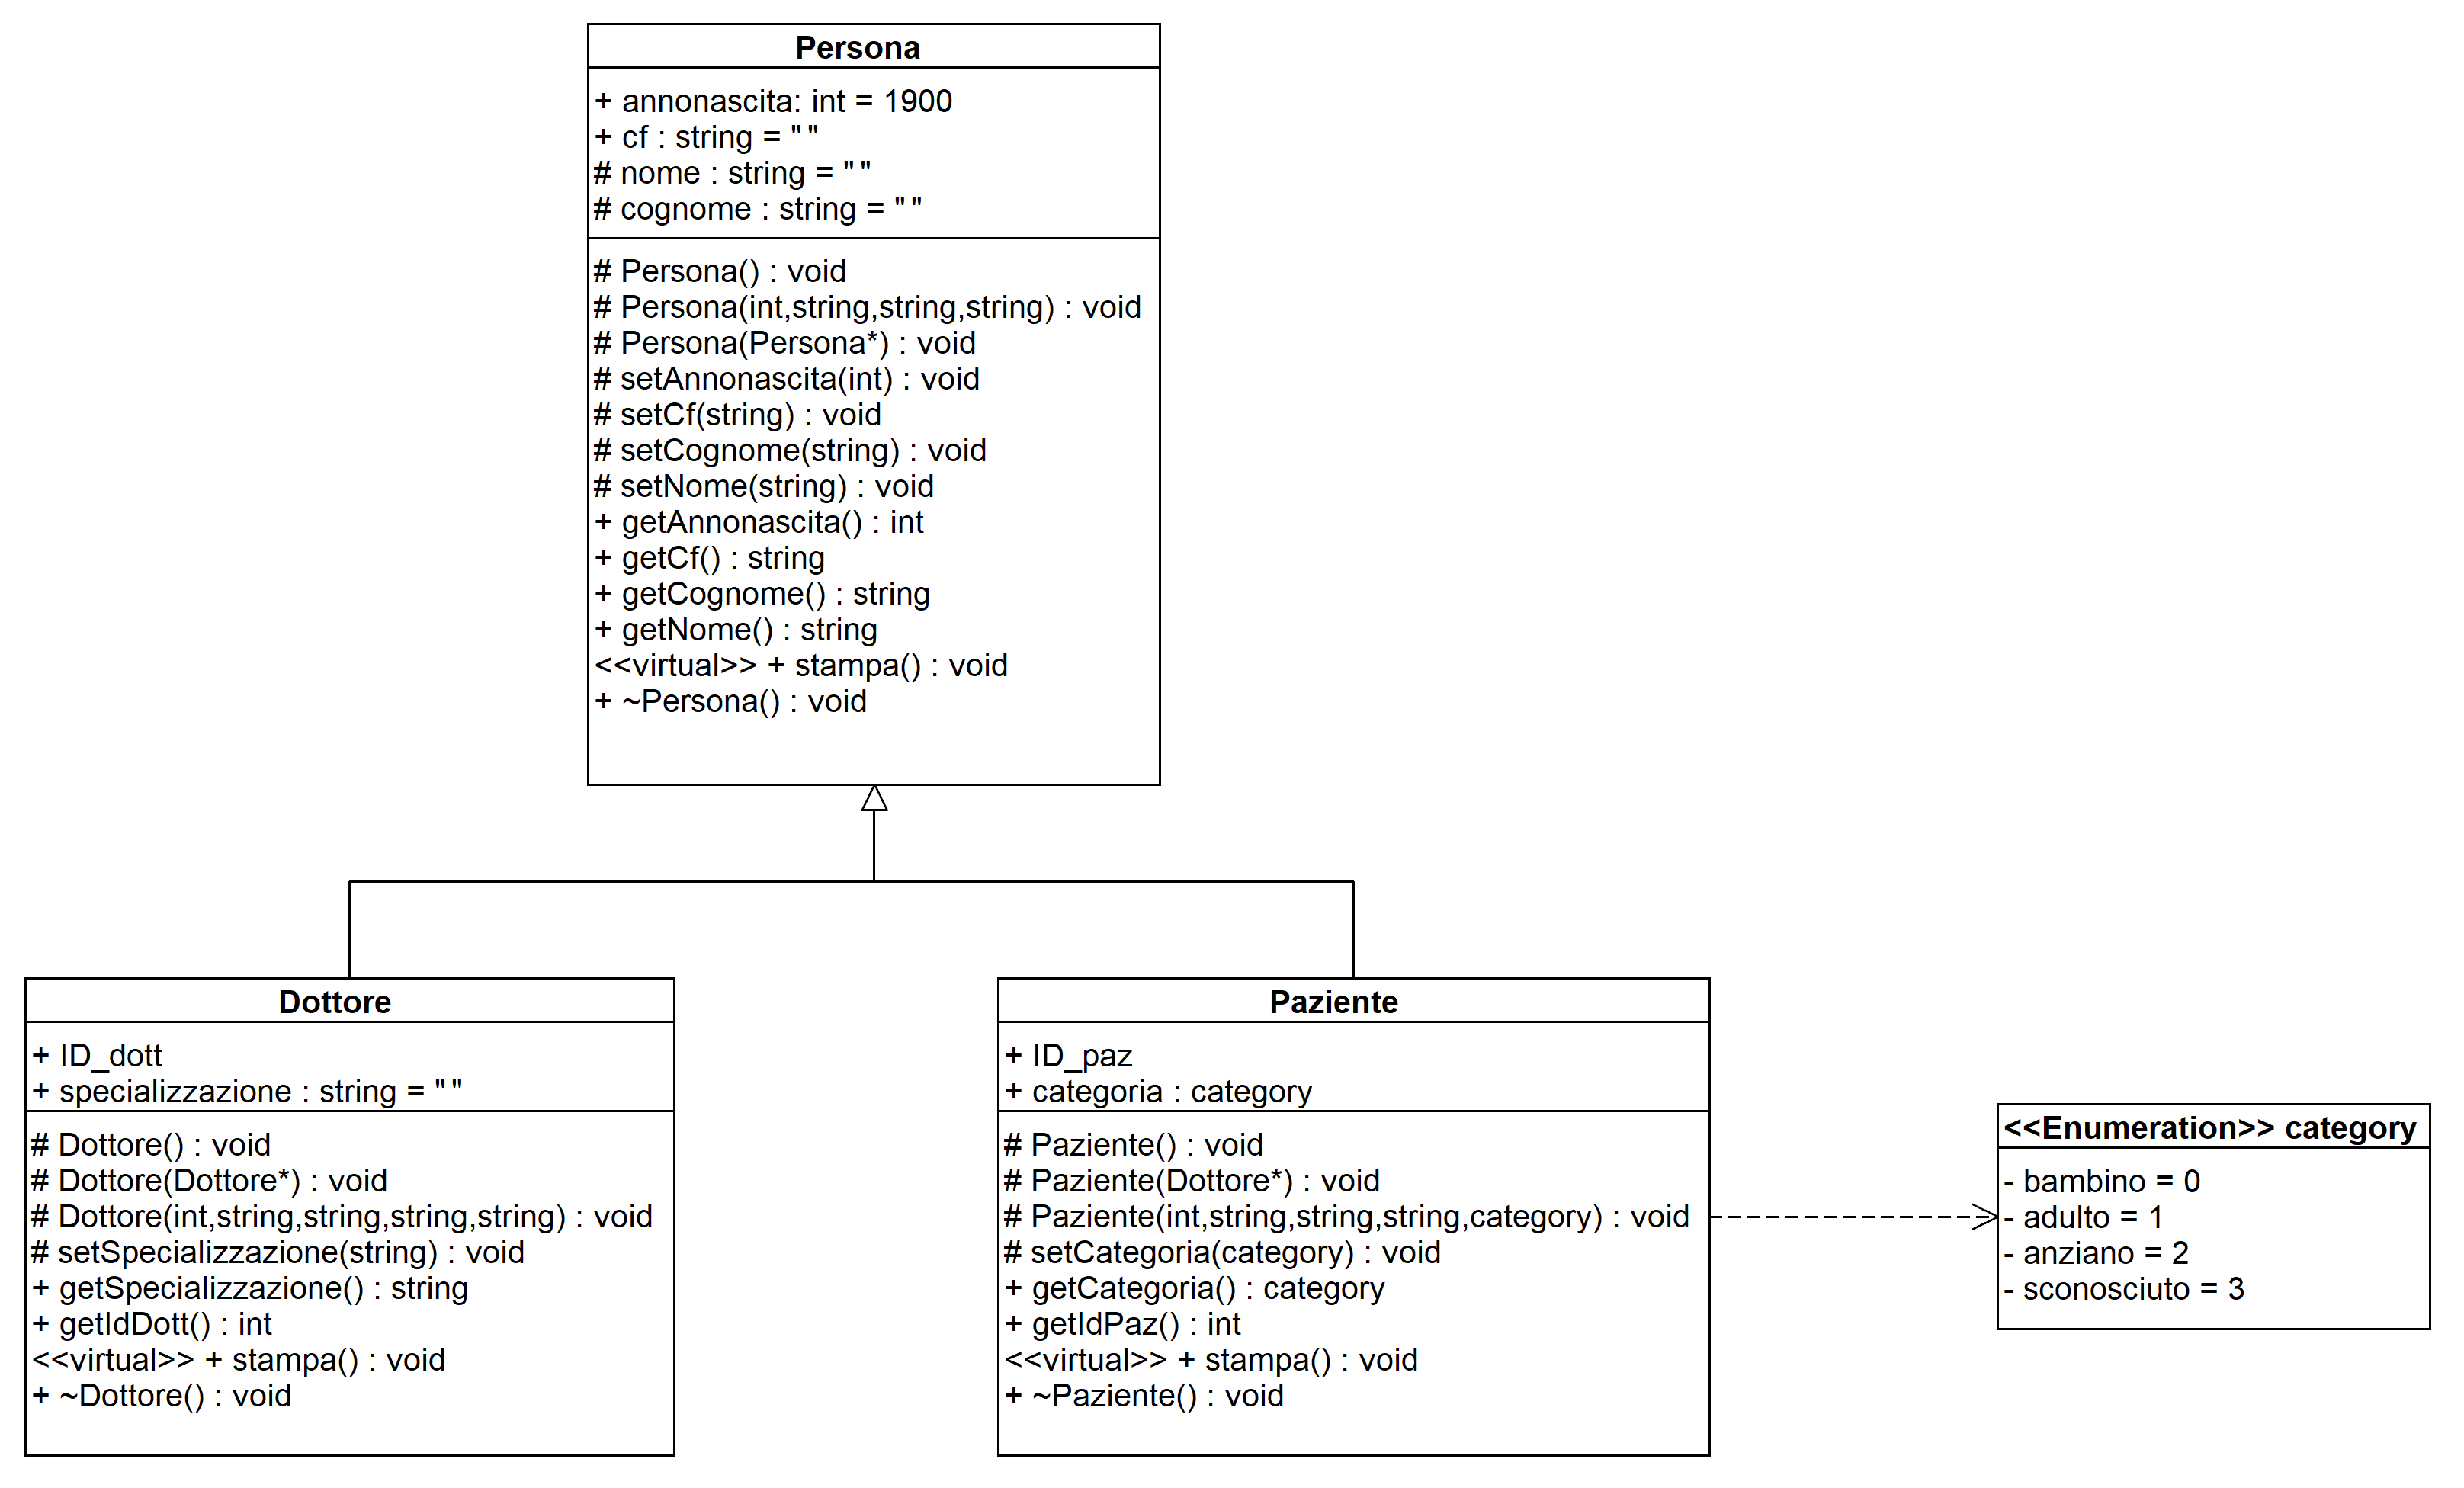
\includegraphics[width=\columnwidth]{diagrammiClassi/gerarchiaPersone}
 \caption{Diagramma delle classi - Gerarchia utenti.}
\end{figure}
\\
\newpage
- Gerarchia delle visite mediche (classi Esame, Pet, Mr e PetMr):\\
\begin{figure}[h]
 \centering
 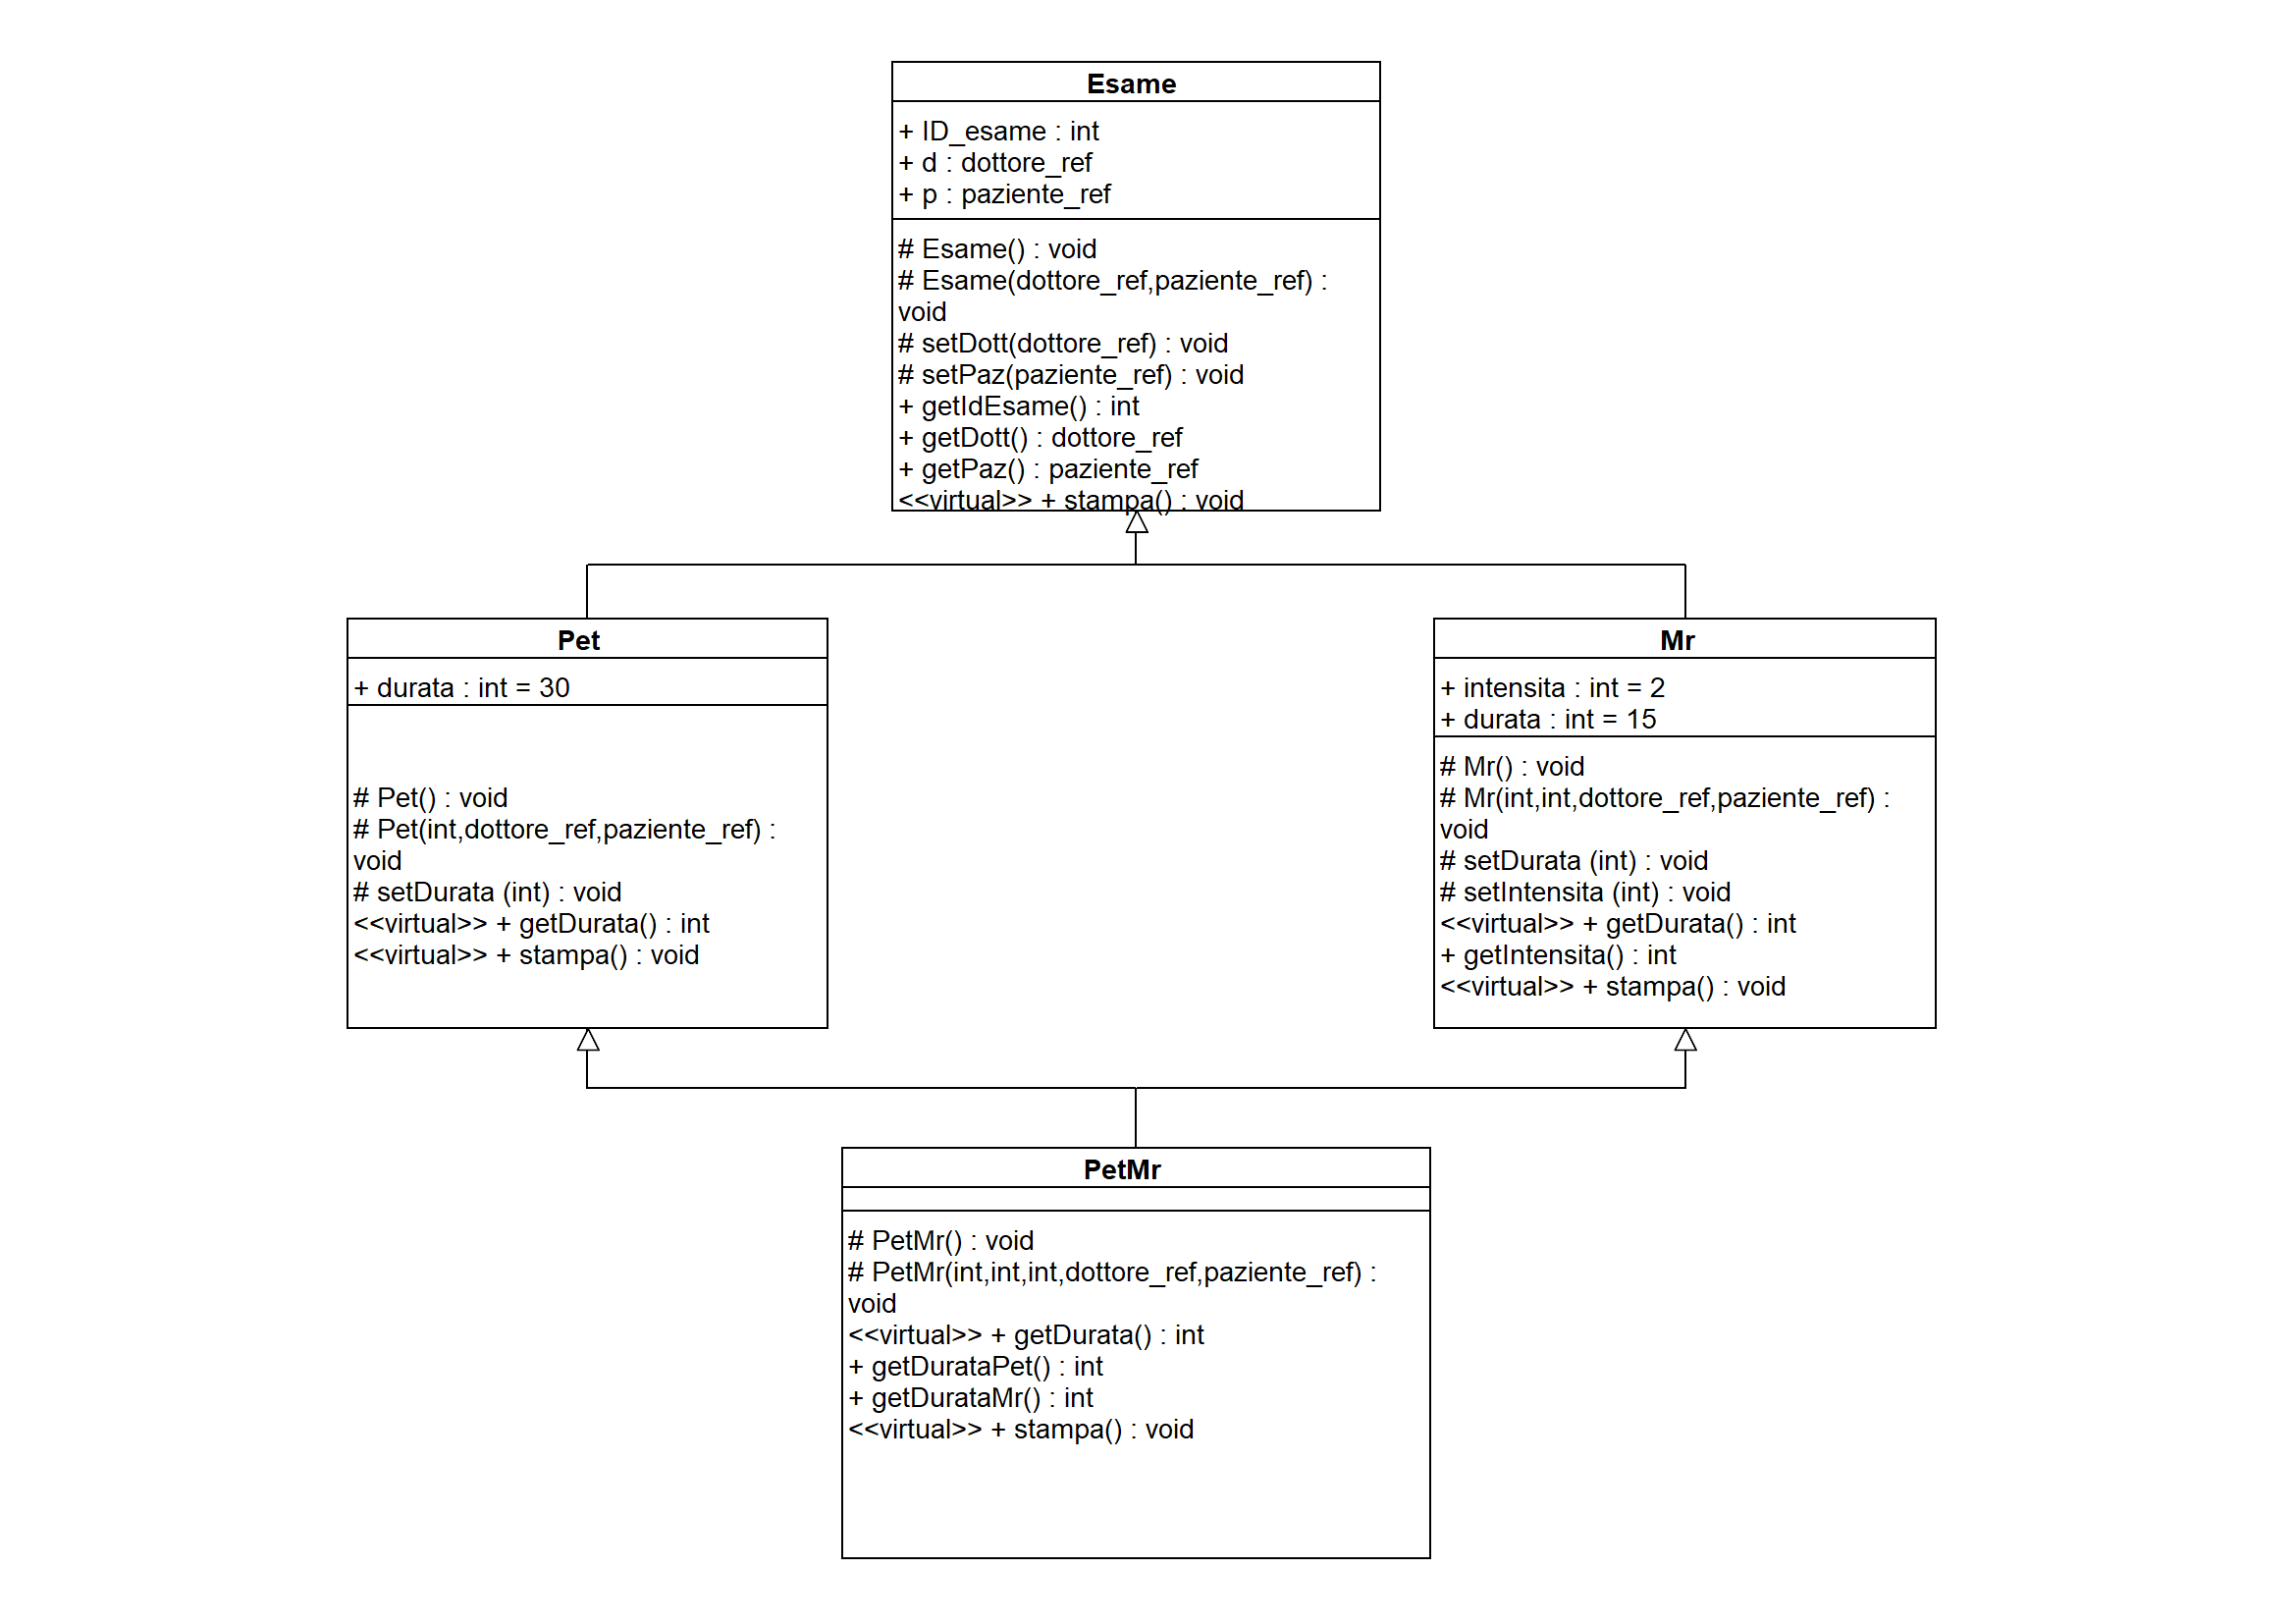
\includegraphics[width=\columnwidth]{diagrammiClassi/gerarchiaEsami}
 \caption{Diagramma delle classi - Gerarchia esami.}
\end{figure}
\\
\newpage
- Interfaccia dei metodi disponibili:
\begin{figure}[h]
 \centering
 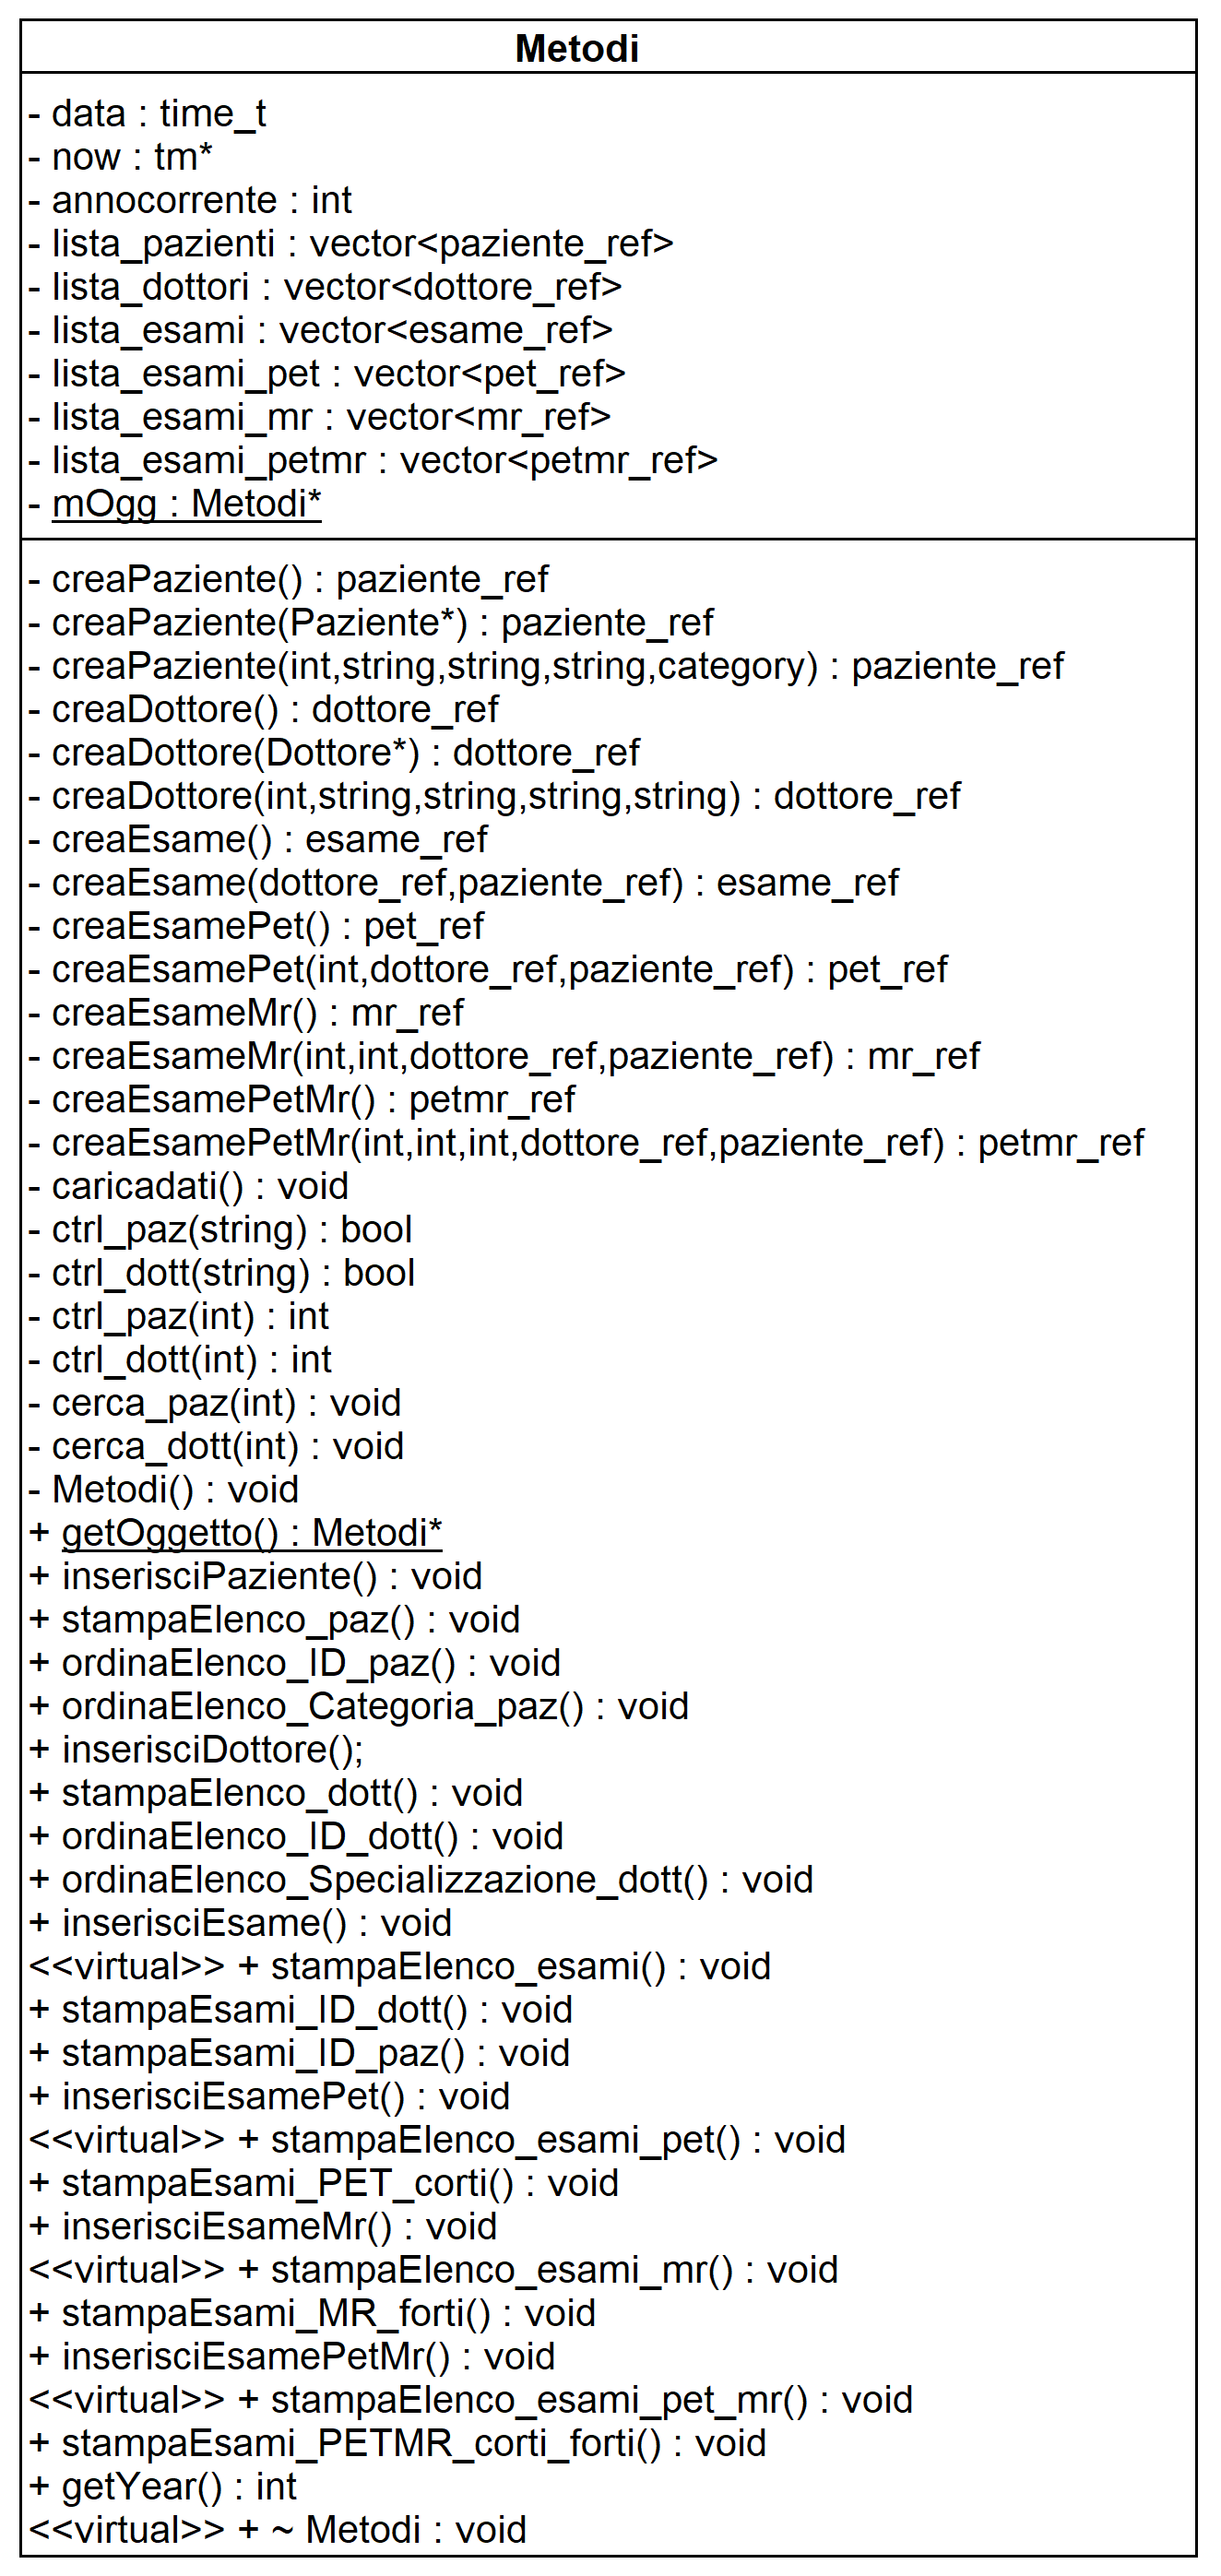
\includegraphics[height=0.73\textheight]{diagrammiClassi/metodi}
 \caption{Diagramma delle classi - Metodi resi disponibili nel programma principale.}
\end{figure}


%----------------------------------------------------------------------------------------
%	CAPITOLO 3
%----------------------------------------------------------------------------------------
\clearpage
\newpage
\section*{Scelte implementative} 
I costruttori sono stati dichiarati \textit{protected}, in modo tale che possano essere richiamati solo dalle classi derivate. Tutte le classi di Utenti e Visite sono \textit{friend} della classe Metodi, in modo tale che la classe di gestione possa accedere a tutti i campi e a tutti i metodi di cui necessita. In questa classe inoltre i metodi che si occupano della creazione di un nuovo oggetto sono stati dichiarati \textit{private}, così che nel main non possano essere richiamati in modo illecito. Anche i metodi utilizzati per il controllo del valore delle variabili sono stati dichiarati \textit{private}, mentre tutti gli altri metodi sono \textit{public}. \\
La classe Metodi ha il costruttore privato perché mette a disposizione una singola istanza che verrà poi utilizzata nel main (design pattern \textit{Singleton}). \\
Per ogni altra classe invece esiste più di un costruttore (\textit{overloading} degli operatori): se non vengono passati i parametri vengono assegnati dei valori di default, in caso contrario si assegnano i parametri passati dall'utente. L'\textit{overloading} viene anche sfruttato nella classe Metodi, nei metodi di creazione di un nuovo oggetto da inserire e nei metodi di controllo. \\
I metodi che si occupano della visualizzazione (stampa) sono stati dichiarati \textit{virtual} per sfruttare il \textit{dinamic binding}: in questo modo viene richiamato il metodo di stampa in base all'oggetto che esegue il metodo e non sulla base del tipo con cui questo oggetto viene dichiarato (a patto che si utilizzino dei puntatori, altrimenti il binding dimanico non verrà eseguito). \\
La gerarchia delle classi che descrivono gli esami forma un diamante, perché sia la classe Pet che la classe Mr hanno come classe base Esame, mentre la classe PetMr eredita sia dalla classe Pet che dalla classe Mr (mediante il meccanismo dell’\textit{ereditarietà multipla} del C++). Per non avere problemi di name clash e duplicazione di campi nella classe derivata PetMr, le classi Pet e Mr ereditano in modo \textit{virtual} dalla classe base Esame.  \\
Al posto di utilizzare i puntatori tradizionali (\textit{raw pointers}), sono stati utilizzati gli \textit{smart pointers} della libreria memory. Questi puntatori si utilizzano come i puntatori raw, ma hanno il vantaggio che il programmatore non deve occuparsi della gestione della memoria come invece avviene per i puntatori tradizionali. Per semplificare il codice, per ogni classe viene dichiarato un tipo di dato che rappresenta uno \textit{shared\_pointer} così da utilizzare poi questo tipo di variabile nel programma. \\
Viene anche utilizzata la libreria STL, in particolare si utilizzano i \textit{vector} come struttura dati per memorizzare la lista di ogni tipo di oggetto (Paziente, Dottore, Esami, Per, Mr e PetMr). Con i \textit{vector} è possibile utilizzare gli \textit{iterator} per scandirli. Gli \textit{iterator} vengono utilizzati nel programma ogni volta che è necessario compiere una detrminata azione su tutti gli elementi della lista, come avviene per esempio nei metodi di stampa. I \textit{vector} possono anche essere ordinati tramite la funzione \textit{sort()}, un algoritmo di ordinamento che richiede tre parametri (il primo e l'ultimo elemento da ordinare e un \textit{comparator}, che indica come va effettuato l'ordinamento). \\
Per le stringhe si utilizza il tipo \textit{string} messo a disposizione dall'omonima libreria, che permette di gestire le stringhe in modo facile e sicuro.






%----------------------------------------------------------------------------------------

}
\end{document}
